\documentclass[a4paper,fleqn]{cas-sc}

\usepackage{iftex}
\ifXeTeX
  \usepackage{fontspec}
  \setmainfont{TeX Gyre Termes}   % font Times ho tro day du tieng Viet
\else
  \usepackage[utf8]{vietnam}      % neu bat buoc dung pdfLaTeX
\fi

\usepackage[numbers]{natbib}
\usepackage{amsmath,amssymb,amsthm}
\usepackage{booktabs,multirow}
\usepackage{xcolor}
\usepackage{graphicx}
\usepackage{tikz}
\usetikzlibrary{arrows.meta,positioning}


\newcommand{\AuthorName}{}
\newcommand{\AuthorEmail}{}
\newcommand{\GithubURL}{}
\IfFileExists{results/author.tex}{\renewcommand{\AuthorName}{An Đức Minh Trí}
\renewcommand{\AuthorEmail}{24021645@vnu.edu.vn}
\renewcommand{\GithubURL}{\url{https://github.com/Her55chers/sudoku-sat}}
}{}
\newcommand{\MachineCPU}{}\newcommand{\MachineCores}{}\newcommand{\MachineRAM}{}
\newcommand{\MachineOS}{}\newcommand{\PythonVersion}{}\newcommand{\TimeLimit}{}
\newcommand{\RepeatText}{}\newcommand{\FixedSolver}{}\newcommand{\BestConfig}{}
\newcommand{\BestSolver}{}\newcommand{\MaxGenN}{}\newcommand{\GenPerCell}{}
\newcommand{\GenSizes}{}\newcommand{\HoleRatios}{}
\newcommand{\AutoAbstract}{}\newcommand{\AutoAmo}{}\newcommand{\AutoSolvers}{}
\newcommand{\AutoScale}{}\newcommand{\AutoConclusion}{}
% TU DONG SINH boi run_experiments.py -- hay doc lai va sua cho tu nhien.
\renewcommand{\MachineCPU}{AMD64 Family 25 Model 97 Stepping 2, AuthenticAMD}
\renewcommand{\MachineCores}{12}
\renewcommand{\MachineRAM}{32 GB}
\renewcommand{\MachineOS}{Windows 11}
\renewcommand{\PythonVersion}{3.14.7}
\renewcommand{\TimeLimit}{200}
\renewcommand{\RepeatText}{Mỗi đề chạy một lần với mỗi cấu hình, chạy song song 6 tiến trình.}
\renewcommand{\FixedSolver}{CaDiCaL}
\renewcommand{\BestConfig}{Pairwise + extended}
\renewcommand{\BestSolver}{CaDiCaL}
\renewcommand{\MaxGenN}{64}
\renewcommand{\GenPerCell}{10}
\renewcommand{\GenSizes}{16, 25, 36, 49, 64}
\renewcommand{\HoleRatios}{0.4, 0.5, 0.6}
\renewcommand{\AutoAbstract}{Trên 150 đề thử nghiệm với giới hạn 200 giây, cấu hình mã hóa tốt nhất là AMO Pairwise với mã hóa extended, và CaDiCaL là solver tốt nhất, giải được 117/150 đề.}
\renewcommand{\AutoAmo}{Với CaDiCaL, cấu hình tốt nhất là Pairwise + extended: giải được 117/150 đề, tổng PAR-2 trên các bộ là 481,49 giây. Cấu hình kém nhất là Binary + minimal (81/150 đề, tổng PAR-2 927,45 giây). Trong 25 cặp (bộ dữ liệu, AMO), mã hóa extended tốt hơn minimal ở 20 cặp, minimal tốt hơn ở 5 cặp, các cặp còn lại như nhau. Trên bộ Gen-64, thứ tự theo thời gian (tốt nhất trước) là Pairwise, Sequential, Binary, Commander, Product, còn thứ tự theo số mệnh đề (ít nhất trước) là Product, Sequential, Commander, Binary, Pairwise; hai thứ tự này không hoàn toàn trùng nhau, nghĩa là kích thước công thức chưa giải thích hết thời gian chạy.}
\renewcommand{\AutoSolvers}{Với cấu hình Pairwise + extended, xếp theo số đề giải được rồi đến PAR-2, thứ tự các solver là CaDiCaL (117/150), CryptoMiniSat (100/150), Glucose (99/150). Solver tốt nhất trên từng bộ: Gen-16: CryptoMiniSat; Gen-25: CryptoMiniSat; Gen-36: CaDiCaL; Gen-49: CaDiCaL; Gen-64: CaDiCaL. So với pairwise + minimal, cấu hình Pairwise + extended tốt hơn với CaDiCaL, Glucose, CryptoMiniSat (3/3 solver), tức là cấu hình tốt nhất tìm được với CaDiCaL cũng có lợi cho các solver khác.}
\renewcommand{\AutoScale}{$N$ lớn nhất mà mỗi solver giải hết các đề trong giới hạn 200 giây (cấu hình Pairwise + extended): CaDiCaL: $25\times25$; Glucose: $25\times25$; CryptoMiniSat: $25\times25$. Với CaDiCaL, thời gian sinh công thức chiếm 40\% tổng thời gian của các đề giải được. Có 5 lần chạy lỗi hoặc hết bộ nhớ (xem cột msg trong \texttt{results/runs.csv}). }
\renewcommand{\AutoConclusion}{Trên 150 đề thử nghiệm với giới hạn 200 giây, cấu hình mã hóa tốt nhất là AMO Pairwise với mã hóa extended, và CaDiCaL là solver tốt nhất, giải được 117/150 đề. Lưới lớn nhất mà CaDiCaL giải hết các đề là $25\times25$.}


%% ---- ten tieng Viet cho bang, hinh, dinh ly ------------------------------
\renewcommand{\tablename}{Bảng}
\renewcommand{\figurename}{Hình}
\renewcommand{\proofname}{Chứng minh}
\makeatletter
\@ifundefined{definition}{\theoremstyle{definition}\newtheorem{definition}{Định nghĩa}}{}
\@ifundefined{proposition}{\theoremstyle{plain}\newtheorem{proposition}{Mệnh đề}}{}
\@ifundefined{remark}{\theoremstyle{remark}\newtheorem{remark}{Nhận xét}}{}
\makeatother

\newcommand{\AMO}{\mathrm{AMO}}
\newcommand{\ALO}{\mathrm{ALO}}
\newcommand{\dom}{\operatorname{dom}}

\begin{document}
\let\WriteBookmarks\relax
\def\floatpagepagefraction{1}
\def\textpagefraction{.001}

\shorttitle{Giải Sudoku bằng SAT}
\shortauthors{\AuthorName}

\title [mode = title]{Giải bài toán Sudoku bằng SAT: so sánh các cách mã hóa AMO và các SAT solver}

\author[1]{\AuthorName , MSV - 24021645}
\cormark[1]
\ead{\AuthorEmail}
\credit{Conceptualization, Methodology, Software, Validation, Writing -- original draft}

\cortext[cor1]{Tác giả liên hệ}

\begin{abstract}
Sudoku là một trò chơi điền số rất quen thuộc. Khi mở rộng lên lưới $N\times N$ (với $N=n^2$) thì bài toán này là NP-đầy đủ. Trong bài tập lớn này, ta xây dựng một bộ giải Sudoku dựa trên SAT: chuyển đề bài thành công thức CNF với $N^3$ biến logic rồi dùng SAT solver để giải. Ta cài đặt hai cách mã hóa là \emph{minimal} và \emph{extended}, và với ràng buộc ``có nhiều nhất một'' (at-most-one, AMO) ta cài đặt năm cách mã hóa: pairwise, sequential counter, binary, commander và product. Ta đưa ra công thức tính số biến và số mệnh đề cho cả mười tổ hợp và kiểm tra lại bằng chương trình. Kết quả cho thấy cách mã hóa AMO ảnh hưởng rất lớn đến kích thước: với lưới $100\times100$, mã hóa minimal cần 148.510.000 mệnh đề nếu dùng pairwise nhưng chỉ cần 8.710.000 mệnh đề nếu dùng product. Công thức CNF được giải và so sánh trên ba SAT solver CaDiCaL, Glucose và CryptoMiniSat. \AutoAbstract
\end{abstract}



\maketitle

%% ============================================================================
\section{Introduction}\label{sec:intro}

Sudoku là trò chơi điền các chữ số từ 1 đến 9 vào một lưới $9\times9$ sao cho mỗi hàng, mỗi cột và mỗi ô vuông $3\times3$ đều chứa đủ các chữ số, mỗi số đúng một lần. Một số ô đã được điền sẵn (gọi là ô cho trước, hay \emph{clue}). Ta có thể mở rộng trò chơi cho lưới $N\times N$ với $N=n^2$ và các khối $n\times n$. Tuy lưới $9\times9$ khá nhỏ, bài toán Sudoku tổng quát đã được chứng minh là NP-đầy đủ~\citep{yato2003}, nên không có thuật toán đa thức nào được biết để giải mọi trường hợp. Các bài toán điền ô kiểu này (hình vuông Latin có lỗ trống) cũng thường được dùng làm bộ dữ liệu kiểm thử cho các thuật toán tìm kiếm~\citep{gomes1997}.

Có ba cách tiếp cận chính xác hay dùng cho Sudoku. Cách thứ nhất là quy hoạch nguyên tuyến tính (ILP), dùng biến nhị phân và các ràng buộc đẳng thức~\citep{bartlett2008}. Cách thứ hai là quy hoạch ràng buộc (CP), dùng một biến nguyên cho mỗi ô cùng ràng buộc \textsc{AllDifferent}~\citep{simonis2005}. Cách thứ ba, và là cách duy nhất được dùng trong bài này, là đưa bài toán về SAT: viết đề bài dưới dạng công thức CNF rồi dùng SAT solver~\citep{weber2005,lynce2006}. Ưu điểm của SAT là tận dụng được các solver CDCL rất mạnh hiện nay. Tuy nhiên người dùng phải tự chọn cách mã hóa các ràng buộc đếm. Trong Sudoku, gần như toàn bộ công thức là ràng buộc AMO: với lưới $9\times9$ mã hóa minimal và AMO pairwise, có 8.748 trên tổng số 8.829 mệnh đề (99,1\%) là mệnh đề AMO. Vì vậy chọn cách mã hóa AMO nào là câu hỏi quan trọng.

Trong bài tập lớn này ta đã làm các việc sau:
\begin{itemize}
\item mô tả hai cách mã hóa minimal và extended cho Sudoku $N\times N$ và giải thích vì sao chúng đúng (Mục~\ref{sec:sat});
\item cài đặt năm cách mã hóa AMO, tính số biến và số mệnh đề của từng cách, và viết chương trình kiểm tra tính đúng đắn (Mục~\ref{sec:amo} và~\ref{sec:validation});
\item viết chương trình giải hoàn chỉnh: sinh CNF, gọi SAT solver qua PySAT~\citep{ignatiev2018}, đọc kết quả, kiểm tra lời giải và kiểm tra lời giải có duy nhất không;
\item so sánh mười cấu hình mã hóa và ba SAT solver (CaDiCaL, Glucose, CryptoMiniSat) trên các đề $9\times9$ và các lưới lớn đến $N=\MaxGenN$ (Mục~\ref{sec:exp}).
\end{itemize}

Phần còn lại của báo cáo gồm: Mục~\ref{sec:background} trình bày bài toán, kiến thức về SAT và các nghiên cứu liên quan; Mục~\ref{sec:sat} trình bày cách mã hóa SAT; Mục~\ref{sec:exp} là thực nghiệm; Mục~\ref{sec:conclusion} là kết luận.

%% ============================================================================
\section{Background}\label{sec:background}

\subsection{Phát biểu bài toán}\label{sec:problem}

Cho $n\ge 2$, $N=n^2$ và $[N]=\{1,\dots,N\}$. Hàng, cột và chữ số được đánh chỉ số bằng $r,c,d\in[N]$. Lưới được chia thành $N$ khối; ô $(r,c)$ thuộc khối
\begin{equation}
b(r,c)=n\left\lfloor \frac{r-1}{n}\right\rfloor+\left\lfloor \frac{c-1}{n}\right\rfloor+1, \label{eq:box}
\end{equation}
và $B_b=\{(r,c): b(r,c)=b\}$ là tập các ô của khối $b$.

\begin{definition}[Sudoku tổng quát]\label{def:sudoku}
Một \emph{lưới Sudoku cấp $n$} là một hàm $S:[N]\times[N]\to[N]$ sao cho mỗi hàng, mỗi cột và mỗi khối chứa mỗi chữ số đúng một lần. Một \emph{đề bài} là một hàm bộ phận $g$ với miền xác định $\dom g\subseteq[N]\times[N]$ (các ô cho trước). Giải đề bài là tìm lưới $S$ thỏa mãn $S(r,c)=g(r,c)$ với mọi $(r,c)\in\dom g$, hoặc chỉ ra rằng không tồn tại lưới như vậy.
\end{definition}

\subsection{SAT, CNF và SAT solver}\label{sec:sat-bg}

Một công thức CNF là hội (AND) của các mệnh đề (clause), mỗi mệnh đề là tuyển (OR) của các literal (biến hoặc phủ định của biến). Bài toán SAT hỏi có tồn tại cách gán giá trị đúng/sai cho các biến để mọi mệnh đề đều đúng hay không. Kỹ thuật cơ bản trong SAT solver là \emph{lan truyền đơn vị} (unit propagation, UP): nếu một mệnh đề chỉ còn đúng một literal chưa gán và các literal khác đều sai thì literal đó buộc phải đúng. Các solver hiện đại theo kiểu CDCL (conflict-driven clause learning) kết hợp UP với việc học mệnh đề mới từ các xung đột và khởi động lại (restart)~\citep{een2003}. Trong bài này ta dùng ba solver: CaDiCaL~\citep{biere2020}, Glucose~\citep{audemard2009} và CryptoMiniSat~\citep{soos2009}. Cả ba đều gọi được trực tiếp từ Python, nên chạy được trên Windows mà không cần công cụ ngoài.

Với tập literal $X=\{x_1,\dots,x_m\}$, $\ALO(X)$ là một mệnh đề duy nhất $x_1\vee\dots\vee x_m$ (ít nhất một biến đúng), còn $\AMO(X)$ yêu cầu có nhiều nhất một biến đúng. Một cách mã hóa AMO có thể thêm các biến phụ $Y$. Ta nói cách mã hóa là \emph{đúng} nếu với mọi cách gán cho $X$, công thức còn thỏa mãn được (bằng cách chọn giá trị cho $Y$) khi và chỉ khi có không quá một $x_i$ đúng.

\subsection{Các nghiên cứu liên quan}\label{sec:related}

\citet{weber2005} là một trong những người đầu tiên giải Sudoku bằng SAT solver. \citet{lynce2006} đề xuất hai cách mã hóa \emph{minimal} và \emph{extended} mà bài này sử dụng; họ nhận thấy với mã hóa extended thì chỉ riêng lan truyền đơn vị đã giải được khoảng một nửa số đề khó trong bộ dữ liệu của họ. Về phía ILP, \citet{bartlett2008} đưa ra mô hình quy hoạch nguyên nhị phân với $N^3$ biến và $4N^2$ ràng buộc đẳng thức. Về phía CP, \citet{simonis2005} mô hình hóa Sudoku bằng \textsc{AllDifferent} và so sánh các mức lan truyền ràng buộc khác nhau.

Về mã hóa AMO, ngoài cách pairwise đơn giản, có sequential counter của \citet{sinz2005} dùng số mệnh đề tuyến tính, commander của \citet{klieber2007} chia biến thành nhóm và thêm một biến ``chỉ huy'' cho mỗi nhóm, product của \citet{chen2010} xếp biến lên một lưới hai chiều, và binary (bitwise) gán cho mỗi biến một mã nhị phân~\citep{frisch2010}. \citet{frisch2010} cũng so sánh nhiều cách mã hóa này với nhau. \citet{kucera2019} chứng minh rằng các mã hóa AMO có tính lan truyền đầy đủ không thể có ít mệnh đề tùy ý, và cận dưới của họ gần với kích thước của các mã hóa tốt nhất đã biết. Các cách mã hóa này cũng đã được áp dụng cho bài toán N-Queens trong một báo cáo trước của môn học~\citep{tran2024nqueens}. Ta chưa tìm thấy tài liệu nào so sánh đồng thời cả năm cách mã hóa AMO trên lưới Sudoku lớn với nhiều SAT solver khác nhau, nên đây là điểm bài này muốn làm.

%% ============================================================================
\section{SAT-based approach}\label{sec:sat}

\subsection{Tổng quan}\label{sec:overview}

Hình~\ref{fig:pipeline} mô tả các bước của chương trình. Bộ mã hóa (encoder) chuyển đề bài $g$ thành công thức CNF $\Phi(g)$ sao cho mỗi mô hình (model) của công thức tương ứng với một lời giải. Công thức được đưa vào SAT solver, hoặc trực tiếp trong bộ nhớ qua PySAT, hoặc qua file DIMACS với solver chạy ngoài. Nếu SAT, mô hình được giải mã thành lưới số, rồi được một hàm kiểm tra độc lập (không dùng chung code với encoder) kiểm tra lại.

\begin{figure}[t]
\centering
\begin{tikzpicture}[node distance=0.5cm, every node/.style={font=\small},
  box/.style={draw, rounded corners=2pt, align=center, minimum height=0.95cm, inner sep=4pt, fill=blue!4},
  arr/.style={-{Stealth[length=2mm]}, thick}]
\node[box] (p) {Đề bài $g$\\(ô cho trước)};
\node[box, right=of p] (e) {Encoder\\(biến thể + AMO)};
\node[box, right=of e] (f) {CNF $\Phi(g)$\\(DIMACS)};
\node[box, right=of f] (s) {SAT solver\\(CDCL)};
\node[box, right=of s] (d) {Giải mã};
\node[box, right=of d] (v) {Kiểm tra\\lời giải};
\draw[arr] (p) -- (e); \draw[arr] (e) -- (f); \draw[arr] (f) -- (s);
\draw[arr] (s) -- node[above, font=\scriptsize]{SAT} (d); \draw[arr] (d) -- (v);
\node[below=0.45cm of s, font=\scriptsize, align=center] (u) {UNSAT $\Rightarrow$ vô nghiệm\\hết giờ $\Rightarrow$ TO};
\draw[arr, dashed] (s) -- (u);
\end{tikzpicture}
\caption{Các bước giải. Bước kiểm tra xác nhận hàng, cột, khối và các ô cho trước của lưới thu được.}
\label{fig:pipeline}
\end{figure}

\subsection{Biến và các nhóm ràng buộc}\label{sec:vars}

Ta dùng mã hóa \emph{trực tiếp} (direct encoding), mỗi cặp (ô, chữ số) có một biến logic:
\begin{equation}
x_{r,c,d}\ \text{đúng}\iff S(r,c)=d,\qquad r,c,d\in[N], \label{eq:var}
\end{equation}
nên có $N^3$ biến chính (729 biến với lưới $9\times9$). Trong file DIMACS, biến $x_{r,c,d}$ có số thứ tự $((r-1)N+(c-1))N+d$. Bảng~\ref{tab:families} liệt kê các nhóm ràng buộc. Mỗi nhóm gồm $N^2$ tập, mỗi tập có đúng $N$ literal: tập của ô $(r,c)$ chạy theo chữ số, tập của $(r,d)$ chạy theo cột, tập của $(c,d)$ chạy theo hàng, và tập của $(b,d)$ chạy theo các ô trong khối $B_b$.

\begin{table}[t]
\caption{Các nhóm ràng buộc trong công thức CNF. Mỗi nhóm có $N^2$ tập gồm $N$ literal. Cột ``M'' và ``E'' cho biết nhóm có mặt trong mã hóa minimal hay extended.}
\label{tab:families}
\centering\small
\begin{tabular}{llccc}
\toprule
Nhóm & Ràng buộc & Số tập & M & E\\
\midrule
(C1) mỗi ô có ít nhất một số & $\ALO(x_{r,c,1},\dots,x_{r,c,N})$ & $N^2$ & \checkmark & \checkmark\\
(C2) mỗi ô có nhiều nhất một số & $\AMO(x_{r,c,1},\dots,x_{r,c,N})$ & $N^2$ & & \checkmark\\
(C3) số $d$ không lặp trong hàng & $\AMO(x_{r,1,d},\dots,x_{r,N,d})$ & $N^2$ & \checkmark & \checkmark\\
(C4) số $d$ không lặp trong cột & $\AMO(x_{1,c,d},\dots,x_{N,c,d})$ & $N^2$ & \checkmark & \checkmark\\
(C5) số $d$ không lặp trong khối & $\AMO(\{x_{r,c,d}:(r,c)\in B_b\})$ & $N^2$ & \checkmark & \checkmark\\
(C6) số $d$ có mặt trong hàng & $\ALO(x_{r,1,d},\dots,x_{r,N,d})$ & $N^2$ & & \checkmark\\
(C7) số $d$ có mặt trong cột & $\ALO(x_{1,c,d},\dots,x_{N,c,d})$ & $N^2$ & & \checkmark\\
(C8) số $d$ có mặt trong khối & $\ALO(\{x_{r,c,d}:(r,c)\in B_b\})$ & $N^2$ & & \checkmark\\
(C9) ô cho trước & mệnh đề đơn $x_{r,c,g(r,c)}$ & $|\dom g|$ & \checkmark & \checkmark\\
\bottomrule
\end{tabular}
\end{table}

Ký hiệu $\Phi_{\mathrm{F}}$ là hội các ràng buộc của nhóm F, hai cách mã hóa là
\begin{align}
\Phi_{\min}(g) &= \Phi_{\mathrm{C1}}\wedge\Phi_{\mathrm{C3}}\wedge\Phi_{\mathrm{C4}}\wedge\Phi_{\mathrm{C5}}\wedge\Phi_{\mathrm{C9}}, \label{eq:min}\\
\Phi_{\mathrm{ext}}(g) &= \Phi_{\min}(g)\wedge\Phi_{\mathrm{C2}}\wedge\Phi_{\mathrm{C6}}\wedge\Phi_{\mathrm{C7}}\wedge\Phi_{\mathrm{C8}}. \label{eq:ext}
\end{align}
Mã hóa minimal đã đủ để mô tả đúng bài toán (Mệnh đề~\ref{prop:sudoku}). Bốn nhóm thêm vào trong extended là thừa về mặt logic, nhưng giúp lan truyền đơn vị suy ra được nhiều hơn. Ví dụ, nếu trong một hàng chỉ còn một ô có thể chứa số $d$ thì mệnh đề (C6) sẽ ép ngay số $d$ vào ô đó.

\begin{proposition}[Tính đúng của mã hóa Sudoku]\label{prop:sudoku}
Giả sử mọi ràng buộc AMO được mã hóa bằng một cách mã hóa đúng. Khi đó với mọi đề bài $g$, các mô hình của $\Phi_{\min}(g)$ (và của $\Phi_{\mathrm{ext}}(g)$), khi chỉ xét các biến chính, tương ứng một-một với các lời giải của $g$ theo quy tắc $S(r,c)=d\iff x_{r,c,d}$.
\end{proposition}

\begin{proof}
Chiều thuận: cho $S$ là một lời giải, đặt $x_{r,c,d}$ đúng khi và chỉ khi $S(r,c)=d$. Khi đó mỗi tập trong mọi nhóm đều có đúng một literal đúng, nên các mệnh đề ALO và mệnh đề đơn đều thỏa mãn, còn các AMO thì thỏa mãn được nhờ chọn giá trị phù hợp cho biến phụ. Vậy phép gán này mở rộng được thành mô hình của $\Phi_{\mathrm{ext}}(g)$, do đó cũng là mô hình của $\Phi_{\min}(g)$.

Chiều ngược: cho $\mu$ là một mô hình của $\Phi_{\min}(g)$. Xét một hàng $r$ và gọi $T_r$ là số cặp $(c,d)$ mà $x_{r,c,d}$ đúng. Theo (C1), mỗi ô trong $N$ ô của hàng có ít nhất một số, nên $T_r\ge N$. Theo (C3), mỗi số trong $N$ số chỉ xuất hiện nhiều nhất ở một ô của hàng, nên $T_r\le N$. Do đó $T_r=N$, nghĩa là mỗi ô của hàng có đúng một số và mỗi số xuất hiện đúng một lần. Điều này đúng với mọi hàng nên $S(r,c)$ được xác định. Với cột $c$: mỗi ô đã có đúng một số, nên có đúng $N$ biến đúng; theo (C4) mỗi số xuất hiện nhiều nhất một lần, nên lập luận đếm như trên cho thấy mỗi số xuất hiện đúng một lần. Khối được xử lý giống hệt nhờ (C5). Các mệnh đề đơn (C9) đảm bảo $S$ khớp với các ô cho trước.
\end{proof}

\subsection{Các cách mã hóa AMO}\label{sec:amo}

Gọi $X=(x_1,\dots,x_m)$ là một tập cần ràng buộc AMO (trong Sudoku $m=N$). Mỗi tập dùng các biến phụ riêng. Ta cài đặt năm cách mã hóa sau; Bảng~\ref{tab:amo} tóm tắt kích thước của chúng.

\paragraph{Pairwise.} Với mọi cặp $i<j$ thêm mệnh đề $(\neg x_i\vee\neg x_j)$. Cách này không cần biến phụ nhưng cần $\binom{m}{2}$ mệnh đề.

\paragraph{Sequential counter~\citep{sinz2005}.} Thêm các biến phụ $s_1,\dots,s_{m-1}$, trong đó $s_i$ có nghĩa ``đã có một $x_j$ đúng với $j\le i$'':
\begin{equation}
(\neg x_1\vee s_1)\wedge\bigwedge_{i=2}^{m-1}\big[(\neg x_i\vee s_i)\wedge(\neg s_{i-1}\vee s_i)\wedge(\neg x_i\vee\neg s_{i-1})\big]\wedge(\neg x_m\vee\neg s_{m-1}). \label{eq:seq}
\end{equation}
Cách này dùng $m-1$ biến phụ và $3m-4$ mệnh đề.

\paragraph{Binary~\citep{frisch2010}.} Đặt $k=\lceil\log_2 m\rceil$ và các biến phụ $y_1,\dots,y_k$. Biến $x_i$ được gán mã nhị phân của $i-1$; ký hiệu $\varphi(i,j)$ là $y_j$ nếu bit thứ $j$ của mã bằng 1, ngược lại là $\neg y_j$:
\begin{equation}
\bigwedge_{i=1}^{m}\bigwedge_{j=1}^{k}\big(\neg x_i\vee\varphi(i,j)\big). \label{eq:bin}
\end{equation}
Cách này dùng $k$ biến phụ và $mk$ mệnh đề.

\paragraph{Commander~\citep{klieber2007}.} Chia $X$ thành $g=\lceil m/3\rceil$ nhóm $G_1,\dots,G_g$ có kích thước gần bằng nhau ($s_i\in\{\lfloor m/g\rfloor,\lceil m/g\rceil\}$). Mỗi nhóm có một biến chỉ huy $c_i$ với $c_i\leftrightarrow\bigvee G_i$:
\begin{equation}
\AMO_{\mathrm{pw}}(c_1,\dots,c_g)\wedge\bigwedge_{i=1}^{g}\Big[\big(\neg c_i\vee\textstyle\bigvee_{x\in G_i}x\big)\wedge\AMO_{\mathrm{pw}}(G_i)\wedge\textstyle\bigwedge_{x\in G_i}(\neg x\vee c_i)\Big], \label{eq:cmd}
\end{equation}
trong đó $\AMO_{\mathrm{pw}}$ là mã hóa pairwise. Ta chỉ dùng một tầng chia nhóm, mỗi nhóm khoảng 3 biến.

\paragraph{Product~\citep{chen2010}.} Đặt $p=\lceil\sqrt m\,\rceil$ và $q=\lceil m/p\rceil$, xếp $x_i$ vào hàng $u_i=\lfloor (i-1)/q\rfloor+1$ và cột $v_i=((i-1)\bmod q)+1$ của một lưới $p\times q$. Với các biến hàng $r_1,\dots,r_p$ và biến cột $c_1,\dots,c_q$:
\begin{equation}
\AMO_{\mathrm{pw}}(r_1,\dots,r_p)\wedge\AMO_{\mathrm{pw}}(c_1,\dots,c_q)\wedge\bigwedge_{i=1}^{m}\big[(\neg x_i\vee r_{u_i})\wedge(\neg x_i\vee c_{v_i})\big]. \label{eq:prod}
\end{equation}
Ở đây ta cũng chỉ dùng một tầng, AMO trên hàng và cột được mã hóa bằng pairwise.

\begin{table}[t]
\caption{Kích thước của một ràng buộc AMO trên $m$ literal. Bốn cột cuối ghi ``số biến phụ / số mệnh đề'' với $m=N\in\{9,16,25,64\}$, do chương trình sinh ra và trùng với công thức ở mọi $2\le m\le 200$.}
\label{tab:amo}
\centering\small
\begin{tabular}{lllcccc}
\toprule
Encoding AMO & Số biến phụ & Số mệnh đề & $m=9$ & $m=16$ & $m=25$ & $m=64$ \\
\midrule
Pairwise & $0$ & $m(m-1)/2$ & 0\,/\,36 & 0\,/\,120 & 0\,/\,300 & 0\,/\,2016 \\
Sequential & $m-1$ & $3m-4$ & 8\,/\,23 & 15\,/\,44 & 24\,/\,71 & 63\,/\,188 \\
Binary & $\lceil\log_2 m\rceil$ & $m\lceil\log_2 m\rceil$ & 4\,/\,36 & 4\,/\,64 & 5\,/\,125 & 6\,/\,384 \\
Commander & $g=\lceil m/3\rceil$ & $\binom{g}{2}+g+m+\sum_i\binom{s_i}{2}$ & 3\,/\,24 & 6\,/\,51 & 9\,/\,93 & 22\,/\,379 \\
Product & $p+q$ & $2m+\binom{p}{2}+\binom{q}{2}$ & 6\,/\,24 & 8\,/\,44 & 10\,/\,70 & 16\,/\,184 \\
\bottomrule
\end{tabular}

\end{table}

\begin{proposition}[Tính đúng]\label{prop:amo}
Cả năm cách trên đều là mã hóa đúng của $\AMO(x_1,\dots,x_m)$.
\end{proposition}

\begin{proposition}[Lan truyền]\label{prop:up}
Với cả năm cách mã hóa và với mọi $i$, nếu gán $x_i=1$ thì lan truyền đơn vị suy ra được $\neg x_j$ cho mọi $j\neq i$ mà không gặp xung đột.
\end{proposition}

Giải thích cho hai mệnh đề này được trình bày ở \ref{app:proofs}. Mệnh đề~\ref{prop:up} cho thấy cả năm cách đều ``loại'' các số còn lại nhanh như pairwise khi một số được đặt vào ô. Điểm khác nhau là số mệnh đề, số biến phụ và độ dài chuỗi suy luận (với sequential counter chuỗi này dài tới $m-1$ bước, các cách khác chỉ vài bước). Cách nào chạy nhanh hơn trên SAT solver thì phải đo bằng thực nghiệm ở Mục~\ref{sec:exp}.

\subsection{Kích thước công thức}\label{sec:size}

\begin{proposition}[Kích thước]\label{prop:size}
Gọi $a(m)$ và $\ell(m)$ là số biến phụ và số mệnh đề của cách mã hóa AMO đã chọn (Bảng~\ref{tab:amo}). Khi đó
\begin{align}
|\mathrm{Var}(\Phi_{\min})| &= N^3+3N^2a(N), & |\Phi_{\min}| &= N^2+3N^2\ell(N)+|\dom g|, \label{eq:size-min}\\
|\mathrm{Var}(\Phi_{\mathrm{ext}})| &= N^3+4N^2a(N), & |\Phi_{\mathrm{ext}}| &= 4N^2+4N^2\ell(N)+|\dom g|. \label{eq:size-ext}
\end{align}
\end{proposition}

\begin{proof}
Mã hóa minimal có một nhóm ALO (C1) và ba nhóm AMO (C3--C5); mã hóa extended có bốn nhóm mỗi loại. Mỗi nhóm có $N^2$ tập; mỗi tập ALO cho một mệnh đề, mỗi tập AMO cho $a(N)$ biến phụ và $\ell(N)$ mệnh đề; mỗi ô cho trước cho một mệnh đề đơn.
\end{proof}

Ví dụ với lưới $9\times9$ và pairwise, công thức \eqref{eq:size-min} cho 729 biến và $81+3\cdot81\cdot36=8.829$ mệnh đề (chưa tính ô cho trước), còn \eqref{eq:size-ext} cho $324+4\cdot81\cdot36=11.988$ mệnh đề. Số mệnh đề tăng theo $\Theta(N^4)$ với pairwise; $\Theta(N^3)$ với sequential counter và product; $\Theta(N^3\log N)$ với binary; còn commander một tầng vẫn là $\Theta(N^4)$ nhưng với hằng số nhỏ hơn nhiều (vì vẫn dùng pairwise trên $\lceil N/3\rceil$ biến chỉ huy).

\subsection{Quy trình giải và kiểm tra nghiệm duy nhất}\label{sec:procedure}

Bảng~\ref{tab:procedure} là quy trình giải đầy đủ. Bước kiểm tra nghiệm duy nhất là tùy chọn, có ích khi sinh đề và khi muốn kiểm tra thêm chương trình.

\begin{table}[t]
\caption{Quy trình giải Sudoku bằng SAT.}
\label{tab:procedure}
\centering\small
\begin{tabular}{p{0.95\linewidth}}
\toprule
\textbf{Đầu vào:} cấp $n$, đề bài $g$, biến thể $\in\{\min,\mathrm{ext}\}$, cách mã hóa AMO, solver, giới hạn thời gian $T$.\\
\textbf{Đầu ra:} lời giải $S$, ``vô nghiệm'' hoặc TO (hết giờ).\\
\midrule
1.\ Sinh $\Phi(g)$ theo \eqref{eq:min} hoặc \eqref{eq:ext}, mỗi tập AMO dùng cách mã hóa đã chọn (Mục~\ref{sec:amo}).\\
2.\ Nạp $\Phi(g)$ vào solver (PySAT) hoặc ghi ra file DIMACS (solver ngoài), gọi \textsc{Solve} với giới hạn $T$.\\
3.\ Nếu UNSAT, trả về ``vô nghiệm''; nếu hết giờ, trả về TO.\\
4.\ Giải mã mô hình: $S(r,c)=d$ với $d$ là số duy nhất mà $x_{r,c,d}$ đúng.\\
5.\ Kiểm tra $S$ bằng hàm kiểm tra độc lập (hàng, cột, khối, ô cho trước); nếu sai nghĩa là chương trình có lỗi.\\
6.\ (Tùy chọn) Thêm mệnh đề chặn $\bigvee_{(r,c)\notin\dom g}\neg x_{r,c,S(r,c)}$ rồi gọi \textsc{Solve} lần nữa; nếu UNSAT thì $S$ là lời giải duy nhất.\\
7.\ Trả về $S$.\\
\bottomrule
\end{tabular}
\end{table}

Mệnh đề chặn ở bước 6 chỉ đúng với các lưới khác $S$ ở ít nhất một ô không cho trước. Vì mỗi mô hình chỉ có một số trong mỗi ô (Mệnh đề~\ref{prop:sudoku}), lần gọi thứ hai trả về UNSAT khi và chỉ khi $S$ là lời giải duy nhất.

Hình~\ref{fig:example} là một đề $9\times9$ có 30 ô cho trước và lời giải mà chương trình tìm được (mã hóa minimal, sequential counter). Khi thêm mệnh đề chặn và giải lại, kết quả là UNSAT, vậy đề này có lời giải duy nhất.

\begin{figure}[t]
\centering
\begin{minipage}[t]{0.47\linewidth}\centering
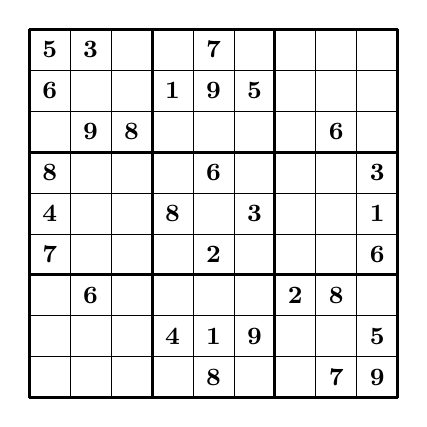
\begin{tikzpicture}[x=0.52cm,y=0.52cm]
\node at (0.5,8.5) {\small\textbf{5}};
\node at (1.5,8.5) {\small\textbf{3}};
\node at (4.5,8.5) {\small\textbf{7}};
\node at (0.5,7.5) {\small\textbf{6}};
\node at (3.5,7.5) {\small\textbf{1}};
\node at (4.5,7.5) {\small\textbf{9}};
\node at (5.5,7.5) {\small\textbf{5}};
\node at (1.5,6.5) {\small\textbf{9}};
\node at (2.5,6.5) {\small\textbf{8}};
\node at (7.5,6.5) {\small\textbf{6}};
\node at (0.5,5.5) {\small\textbf{8}};
\node at (4.5,5.5) {\small\textbf{6}};
\node at (8.5,5.5) {\small\textbf{3}};
\node at (0.5,4.5) {\small\textbf{4}};
\node at (3.5,4.5) {\small\textbf{8}};
\node at (5.5,4.5) {\small\textbf{3}};
\node at (8.5,4.5) {\small\textbf{1}};
\node at (0.5,3.5) {\small\textbf{7}};
\node at (4.5,3.5) {\small\textbf{2}};
\node at (8.5,3.5) {\small\textbf{6}};
\node at (1.5,2.5) {\small\textbf{6}};
\node at (6.5,2.5) {\small\textbf{2}};
\node at (7.5,2.5) {\small\textbf{8}};
\node at (3.5,1.5) {\small\textbf{4}};
\node at (4.5,1.5) {\small\textbf{1}};
\node at (5.5,1.5) {\small\textbf{9}};
\node at (8.5,1.5) {\small\textbf{5}};
\node at (4.5,0.5) {\small\textbf{8}};
\node at (7.5,0.5) {\small\textbf{7}};
\node at (8.5,0.5) {\small\textbf{9}};
\draw[line width=1.1pt] (0,0) -- (9,0); \draw[line width=1.1pt] (0,0) -- (0,9);
\draw[line width=0.3pt] (0,1) -- (9,1); \draw[line width=0.3pt] (1,0) -- (1,9);
\draw[line width=0.3pt] (0,2) -- (9,2); \draw[line width=0.3pt] (2,0) -- (2,9);
\draw[line width=1.1pt] (0,3) -- (9,3); \draw[line width=1.1pt] (3,0) -- (3,9);
\draw[line width=0.3pt] (0,4) -- (9,4); \draw[line width=0.3pt] (4,0) -- (4,9);
\draw[line width=0.3pt] (0,5) -- (9,5); \draw[line width=0.3pt] (5,0) -- (5,9);
\draw[line width=1.1pt] (0,6) -- (9,6); \draw[line width=1.1pt] (6,0) -- (6,9);
\draw[line width=0.3pt] (0,7) -- (9,7); \draw[line width=0.3pt] (7,0) -- (7,9);
\draw[line width=0.3pt] (0,8) -- (9,8); \draw[line width=0.3pt] (8,0) -- (8,9);
\draw[line width=1.1pt] (0,9) -- (9,9); \draw[line width=1.1pt] (9,0) -- (9,9);
\end{tikzpicture}
\\[2pt] (a) đề bài (30 ô cho trước)
\end{minipage}\hfill
\begin{minipage}[t]{0.47\linewidth}\centering
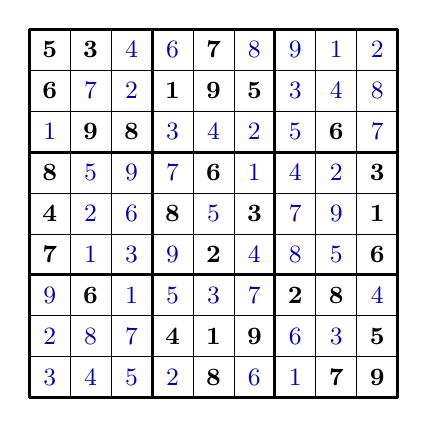
\begin{tikzpicture}[x=0.52cm,y=0.52cm]
\node at (0.5,8.5) {\small\textbf{5}};
\node at (1.5,8.5) {\small\textbf{3}};
\node[blue!70!black] at (2.5,8.5) {\small 4};
\node[blue!70!black] at (3.5,8.5) {\small 6};
\node at (4.5,8.5) {\small\textbf{7}};
\node[blue!70!black] at (5.5,8.5) {\small 8};
\node[blue!70!black] at (6.5,8.5) {\small 9};
\node[blue!70!black] at (7.5,8.5) {\small 1};
\node[blue!70!black] at (8.5,8.5) {\small 2};
\node at (0.5,7.5) {\small\textbf{6}};
\node[blue!70!black] at (1.5,7.5) {\small 7};
\node[blue!70!black] at (2.5,7.5) {\small 2};
\node at (3.5,7.5) {\small\textbf{1}};
\node at (4.5,7.5) {\small\textbf{9}};
\node at (5.5,7.5) {\small\textbf{5}};
\node[blue!70!black] at (6.5,7.5) {\small 3};
\node[blue!70!black] at (7.5,7.5) {\small 4};
\node[blue!70!black] at (8.5,7.5) {\small 8};
\node[blue!70!black] at (0.5,6.5) {\small 1};
\node at (1.5,6.5) {\small\textbf{9}};
\node at (2.5,6.5) {\small\textbf{8}};
\node[blue!70!black] at (3.5,6.5) {\small 3};
\node[blue!70!black] at (4.5,6.5) {\small 4};
\node[blue!70!black] at (5.5,6.5) {\small 2};
\node[blue!70!black] at (6.5,6.5) {\small 5};
\node at (7.5,6.5) {\small\textbf{6}};
\node[blue!70!black] at (8.5,6.5) {\small 7};
\node at (0.5,5.5) {\small\textbf{8}};
\node[blue!70!black] at (1.5,5.5) {\small 5};
\node[blue!70!black] at (2.5,5.5) {\small 9};
\node[blue!70!black] at (3.5,5.5) {\small 7};
\node at (4.5,5.5) {\small\textbf{6}};
\node[blue!70!black] at (5.5,5.5) {\small 1};
\node[blue!70!black] at (6.5,5.5) {\small 4};
\node[blue!70!black] at (7.5,5.5) {\small 2};
\node at (8.5,5.5) {\small\textbf{3}};
\node at (0.5,4.5) {\small\textbf{4}};
\node[blue!70!black] at (1.5,4.5) {\small 2};
\node[blue!70!black] at (2.5,4.5) {\small 6};
\node at (3.5,4.5) {\small\textbf{8}};
\node[blue!70!black] at (4.5,4.5) {\small 5};
\node at (5.5,4.5) {\small\textbf{3}};
\node[blue!70!black] at (6.5,4.5) {\small 7};
\node[blue!70!black] at (7.5,4.5) {\small 9};
\node at (8.5,4.5) {\small\textbf{1}};
\node at (0.5,3.5) {\small\textbf{7}};
\node[blue!70!black] at (1.5,3.5) {\small 1};
\node[blue!70!black] at (2.5,3.5) {\small 3};
\node[blue!70!black] at (3.5,3.5) {\small 9};
\node at (4.5,3.5) {\small\textbf{2}};
\node[blue!70!black] at (5.5,3.5) {\small 4};
\node[blue!70!black] at (6.5,3.5) {\small 8};
\node[blue!70!black] at (7.5,3.5) {\small 5};
\node at (8.5,3.5) {\small\textbf{6}};
\node[blue!70!black] at (0.5,2.5) {\small 9};
\node at (1.5,2.5) {\small\textbf{6}};
\node[blue!70!black] at (2.5,2.5) {\small 1};
\node[blue!70!black] at (3.5,2.5) {\small 5};
\node[blue!70!black] at (4.5,2.5) {\small 3};
\node[blue!70!black] at (5.5,2.5) {\small 7};
\node at (6.5,2.5) {\small\textbf{2}};
\node at (7.5,2.5) {\small\textbf{8}};
\node[blue!70!black] at (8.5,2.5) {\small 4};
\node[blue!70!black] at (0.5,1.5) {\small 2};
\node[blue!70!black] at (1.5,1.5) {\small 8};
\node[blue!70!black] at (2.5,1.5) {\small 7};
\node at (3.5,1.5) {\small\textbf{4}};
\node at (4.5,1.5) {\small\textbf{1}};
\node at (5.5,1.5) {\small\textbf{9}};
\node[blue!70!black] at (6.5,1.5) {\small 6};
\node[blue!70!black] at (7.5,1.5) {\small 3};
\node at (8.5,1.5) {\small\textbf{5}};
\node[blue!70!black] at (0.5,0.5) {\small 3};
\node[blue!70!black] at (1.5,0.5) {\small 4};
\node[blue!70!black] at (2.5,0.5) {\small 5};
\node[blue!70!black] at (3.5,0.5) {\small 2};
\node at (4.5,0.5) {\small\textbf{8}};
\node[blue!70!black] at (5.5,0.5) {\small 6};
\node[blue!70!black] at (6.5,0.5) {\small 1};
\node at (7.5,0.5) {\small\textbf{7}};
\node at (8.5,0.5) {\small\textbf{9}};
\draw[line width=1.1pt] (0,0) -- (9,0); \draw[line width=1.1pt] (0,0) -- (0,9);
\draw[line width=0.3pt] (0,1) -- (9,1); \draw[line width=0.3pt] (1,0) -- (1,9);
\draw[line width=0.3pt] (0,2) -- (9,2); \draw[line width=0.3pt] (2,0) -- (2,9);
\draw[line width=1.1pt] (0,3) -- (9,3); \draw[line width=1.1pt] (3,0) -- (3,9);
\draw[line width=0.3pt] (0,4) -- (9,4); \draw[line width=0.3pt] (4,0) -- (4,9);
\draw[line width=0.3pt] (0,5) -- (9,5); \draw[line width=0.3pt] (5,0) -- (5,9);
\draw[line width=1.1pt] (0,6) -- (9,6); \draw[line width=1.1pt] (6,0) -- (6,9);
\draw[line width=0.3pt] (0,7) -- (9,7); \draw[line width=0.3pt] (7,0) -- (7,9);
\draw[line width=0.3pt] (0,8) -- (9,8); \draw[line width=0.3pt] (8,0) -- (8,9);
\draw[line width=1.1pt] (0,9) -- (9,9); \draw[line width=1.1pt] (9,0) -- (9,9);
\end{tikzpicture}
\\[2pt] (b) lời giải đọc từ mô hình SAT
\end{minipage}

\caption{Ví dụ đề $9\times9$. Số in đậm là ô cho trước, số màu xanh là số do solver điền.}
\label{fig:example}
\end{figure}

%% ============================================================================
\section{Computational experiments}\label{sec:exp}

\subsection{Môi trường thực nghiệm}\label{sec:setup}

Các thí nghiệm chạy trên máy có CPU \MachineCPU{} (\MachineCores{} luồng), RAM \MachineRAM, hệ điều hành \MachineOS, Python \PythonVersion. Mỗi SAT solver chạy một luồng, giới hạn thời gian \TimeLimit~giây. \RepeatText{} Để tránh solver treo, mỗi lần chạy là một tiến trình riêng và bị dừng nếu quá giới hạn. Thời gian ghi lại là thời gian thực của cả lần chạy, gồm sinh công thức, gọi solver và giải mã; nếu quá giới hạn thì ghi là TO. Bảng~\ref{tab:solvers} liệt kê các SAT solver. Khi tổng hợp kết quả, ta ghi số đề giải được và điểm PAR-2 (thời gian trung bình, trong đó mỗi lần TO được tính bằng hai lần giới hạn thời gian), đồng thời vẽ biểu đồ cactus để xem phân bố thời gian.

\begin{table}[t]
\caption{Các SAT solver và cách gọi. ``không chạy'' nghĩa là solver không cài được trên máy thử nghiệm.}
\label{tab:solvers}
\centering\small
\begin{tabular}{lll}
\toprule
Solver & Cách gọi & Phiên bản\\
\midrule
CaDiCaL~\citep{biere2020} & PySAT (\texttt{cadical195}) & 1.9.5 (PySAT 1.9.dev16)\\
Glucose~\citep{audemard2009} & PySAT (\texttt{glucose4}) & 4.1 (PySAT 1.9.dev16)\\
CryptoMiniSat~\citep{soos2009} & file chạy \texttt{cryptominisat5}, đọc DIMACS & --\\
\midrule
OR-Tools CP-SAT~\citep{cpsat} & \texttt{ortools}, mô hình CP (\textsc{AllDifferent}) & OR-Tools 9.15.6755\\
\bottomrule
\end{tabular}

\end{table}

\subsection{Bộ dữ liệu}\label{sec:bench}

Ta dùng hai nhóm dữ liệu (Bảng~\ref{tab:bench}). Nhóm thứ nhất là các đề $9\times9$ khó đã được công bố: bộ \emph{top95} (95 đề) và \emph{hardest} (11 đề) của~\citet{norvig}. Nhóm thứ hai là các đề do ta tự sinh với $N\in\{\GenSizes\}$. Cách sinh như sau: lấy một lưới hợp lệ theo mẫu, hoán vị ngẫu nhiên các chữ số, các hàng trong từng dải, các dải, các cột trong từng cột khối và các cột khối, sau đó xóa ngẫu nhiên một tỉ lệ $h$ số ô. Đề sinh theo cách này chắc chắn có lời giải nhưng có thể có nhiều lời giải. Ta dùng $h\in\{\HoleRatios\}$ vì các bài toán điền hình vuông Latin thường khó nhất ở vùng tỉ lệ ô trống trung bình~\citep{gomes1997}, mỗi cặp $(N,h)$ sinh \GenPerCell{} đề với seed cố định.

\begin{table}[t]
\caption{Các bộ dữ liệu.}
\label{tab:bench}
\centering\small
\begin{tabular}{llcc}
\toprule
Bộ & Nguồn & $N$ & Số đề\\
\midrule
Gen-36 & tự sinh, 10 đề mỗi $h$ & 36 & 30\\
\bottomrule
\end{tabular}

\end{table}

\subsection{Kích thước công thức}\label{sec:exp-size}

Bảng~\ref{tab:size-min} và Hình~\ref{fig:size} cho kích thước của mã hóa minimal với $N$ từ 9 đến 100 (mã hóa extended ở \ref{app:tables}). Các số này tính theo Mệnh đề~\ref{prop:size}; với $N\le49$ ta đã đếm lại trực tiếp số mệnh đề do encoder sinh ra và thấy trùng khớp (Mục~\ref{sec:validation}).

\begin{table}[t]
\caption{Mã hóa minimal (chưa tính ô cho trước): (a) số biến, (b) số mệnh đề. Giá trị nhỏ nhất trên mỗi hàng được in đậm.}
\label{tab:size-min}
\centering\small
(a) Số biến\par\smallskip
\begin{tabular}{rrrrrr}
\toprule
$N$ & Pairwise & Sequential & Binary & Commander & Product \\
\midrule
9 & \textbf{729} & 2\,673 & 1\,701 & 1\,458 & 2\,187 \\
16 & \textbf{4\,096} & 15\,616 & 7\,168 & 8\,704 & 10\,240 \\
25 & \textbf{15\,625} & 60\,625 & 25\,000 & 32\,500 & 34\,375 \\
36 & \textbf{46\,656} & 182\,736 & 69\,984 & 93\,312 & 93\,312 \\
49 & \textbf{117\,649} & 463\,393 & 160\,867 & 240\,100 & 218\,491 \\
64 & \textbf{262\,144} & 1\,036\,288 & 335\,872 & 532\,480 & 458\,752 \\
100 & \textbf{1\,000\,000} & 3\,970\,000 & 1\,210\,000 & 2\,020\,000 & 1\,600\,000 \\
\bottomrule
\end{tabular}
\par\bigskip
(b) Số mệnh đề\par\smallskip
\begin{tabular}{rrrrrr}
\toprule
$N$ & Pairwise & Sequential & Binary & Commander & Product \\
\midrule
9 & 8\,829 & \textbf{5\,670} & 8\,829 & 5\,913 & 5\,913 \\
16 & 92\,416 & \textbf{34\,048} & 49\,408 & 39\,424 & \textbf{34\,048} \\
25 & 563\,125 & 133\,750 & 235\,000 & 175\,000 & \textbf{131\,875} \\
36 & 2\,450\,736 & 405\,648 & 841\,104 & 584\,496 & \textbf{397\,872} \\
49 & 8\,473\,129 & 1\,032\,430 & 2\,120\,083 & 1\,795\,948 & \textbf{1\,010\,821} \\
64 & 24\,776\,704 & 2\,314\,240 & 4\,722\,688 & 4\,661\,248 & \textbf{2\,265\,088} \\
100 & 148\,510\,000 & 8\,890\,000 & 21\,010\,000 & 23\,800\,000 & \textbf{8\,710\,000} \\
\bottomrule
\end{tabular}

\end{table}

\begin{figure}[t]
\centering
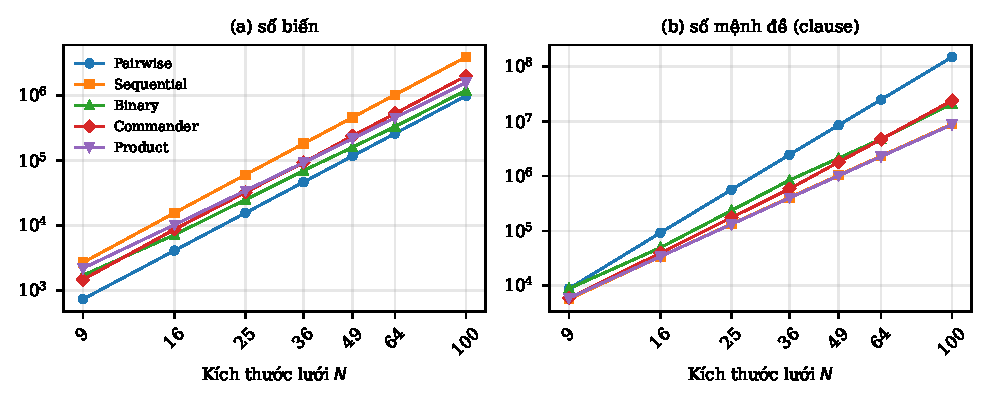
\includegraphics[width=0.92\linewidth]{figures/encoding_size.pdf}
\caption{Kích thước mã hóa minimal theo $N$ (thang log--log).}
\label{fig:size}
\end{figure}

Từ bảng và hình có thể thấy mấy điểm sau. Thứ nhất, pairwise là cách duy nhất không cần biến phụ, nhưng số mệnh đề tăng nhanh nhất: từ 8.829 ở $N=9$ lên 148.510.000 ở $N=100$, gấp khoảng 17 lần product. Từ $N=64$ lên $N=100$ số mệnh đề của pairwise tăng 5,99 lần, gần với $(100/64)^4\approx5{,}96$, còn của product tăng 3,85 lần, gần với $(100/64)^3\approx3{,}81$. Thứ hai, ở $N=9$ sequential counter cho ít mệnh đề nhất (5.670, ít hơn pairwise 35,8\%), còn từ $N=25$ trở đi product cho ít mệnh đề nhất, nhưng chỉ hơn sequential counter một chút (1,4\% ở $N=25$ và 2,0\% ở $N=100$). Thứ ba, sequential counter phải trả giá bằng số biến lớn nhất, gần gấp bốn pairwise ở $N=100$ (3.970.000 so với 1.000.000). Binary thì ngược lại: chỉ thêm 21\% số biến ở $N=100$ nhưng có số mệnh đề gấp 2,4 lần product. Cuối cùng, ở $N=9$ binary và pairwise có số mệnh đề bằng nhau ($9\cdot\lceil\log_2 9\rceil=36=\binom{9}{2}$), nên trên Sudoku thường binary không giảm được mệnh đề nào mà chỉ thêm biến. Tuy vậy, thời gian chạy của SAT solver không chỉ phụ thuộc vào kích thước, nên các con số này chỉ là điểm xuất phát cho các thí nghiệm bên dưới.

\subsection{Kiểm tra tính đúng}\label{sec:validation}

Trước khi đo thời gian, ta kiểm tra encoder bằng các bài kiểm tra trong Bảng~\ref{tab:validation}. Các bài kiểm tra dùng một bộ giải DPLL nhỏ viết kèm trong code, độc lập với các solver CDCL ở Bảng~\ref{tab:solvers}. Tất cả đều đạt.

\begin{table}[t]
\caption{Các bài kiểm tra (tất cả đều đạt). Số trường hợp tính cho mỗi cách mã hóa AMO, trừ khi ghi ``tổng''.}
\label{tab:validation}
\centering\small
\begin{tabular}{p{0.66\linewidth}r}
\toprule
Bài kiểm tra & Số trường hợp\\
\midrule
AMO, vét cạn: mọi $2^m$ cách gán cho $x_1,\dots,x_m$ với $m=1,\dots,10$; SAT khi và chỉ khi có nhiều nhất một biến đúng & 2.046\\
AMO, mọi cách gán có 0, 1 hoặc 2 biến đúng, $m=11,\dots,24$ & 2.394\\
Tính lan truyền (Mệnh đề~\ref{prop:up}): UP từ $x_i=1$, $m=2,\dots,64$, mọi $i$ & 2.079\\
Công thức kích thước AMO (Bảng~\ref{tab:amo}) so với chương trình, $m=2,\dots,200$ & 199\\
Công thức kích thước Sudoku (Mệnh đề~\ref{prop:size}) so với chương trình, $N\in\{4,9,\dots,49\}$, 5 AMO $\times$ 2 biến thể (tổng) & 60\\
Đề ở Hình~\ref{fig:example}, 5 AMO $\times$ 2 biến thể: lời giải hợp lệ và trùng đáp án (tổng) & 10\\
Kiểm tra nghiệm duy nhất của đề ở Hình~\ref{fig:example} (mệnh đề chặn cho UNSAT) & 1\\
Lưới $4\times4$ trống là SAT; hai ô cùng số trong một hàng là UNSAT (tổng) & 2\\
Đề tự sinh với $N\in\{4,9,16\}$, lời giải qua được hàm kiểm tra (tổng) & 15\\
\bottomrule
\end{tabular}
\end{table}

\subsection{Ảnh hưởng của cách mã hóa AMO}\label{sec:exp-amo}

Bảng~\ref{tab:res-amo} so sánh mười cấu hình mã hóa khi dùng cùng một solver (\FixedSolver). \AutoAmo

\begin{table}[t]
\caption{Ảnh hưởng của cách mã hóa AMO với \FixedSolver: số đề giải được / tổng số đề (PAR-2, giây). Ô in đậm là tốt nhất trên mỗi hàng.}
\label{tab:res-amo}
\centering\small
\begin{tabular}{llccccc}
\toprule
Bộ & Biến thể & Pairwise & Sequential & Binary & Commander & Product \\
\midrule
\multirow{2}{*}{Gen-36} & minimal & \textbf{22/30 (136,4)} & 15/30 (210,9) & 11/30 (258,0) & 16/30 (204,4) & 17/30 (204,1) \\
 & extended & 26/30 (57,96) & \textbf{27/30 (50,15)} & 25/30 (72,39) & 27/30 (51,69) & 26/30 (58,37) \\
\bottomrule
\end{tabular}

\end{table}

\subsection{So sánh các SAT solver}\label{sec:exp-solvers}

Bảng~\ref{tab:res-solvers} so sánh ba SAT solver với hai cấu hình: cấu hình tốt nhất ở Bảng~\ref{tab:res-amo} và cấu hình đơn giản nhất (pairwise + minimal), để xem cấu hình tốt cho \FixedSolver{} có tốt cho các solver khác hay không. Hình~\ref{fig:cactus} vẽ phân bố thời gian của các solver với cấu hình tốt nhất. \AutoSolvers{} Lưu ý rằng nếu CryptoMiniSat được gọi bằng file chạy riêng thay vì \texttt{pycryptosat}, thời gian của nó còn gồm cả việc ghi file DIMACS.

\begin{table}[t]
\caption{Các SAT solver với cấu hình tốt nhất (\BestConfig) và với pairwise + minimal: số đề giải được / tổng số đề (PAR-2, giây). Ô in đậm là solver tốt nhất trên mỗi cột trong cùng cấu hình.}
\label{tab:res-solvers}
\centering\small
\begin{tabular}{llccccc}
\toprule
Cấu hình & Solver & Gen-16 & Gen-25 & Gen-36 & Gen-49 & Gen-64 \\
\midrule
\multirow{3}{*}{\shortstack[l]{Pairwise\\extended}} & CaDiCaL & 30/30 (0,15) & 30/30 (0,71) & \textbf{26/30 (57,96)} & \textbf{20/30 (141,1)} & \textbf{11/30 (281,6)} \\
 & Glucose & 30/30 (0,09) & 30/30 (0,44) & 26/30 (60,97) & 13/30 (236,7) & 0/30 (400,0) \\
 & CryptoMiniSat & \textbf{30/30 (0,07)} & \textbf{30/30 (0,42)} & 26/30 (58,21) & 14/30 (219,7) & 0/30 (400,0) \\
\midrule
\multirow{3}{*}{\shortstack[l]{Pairwise\\minimal}} & CaDiCaL & 30/30 (0,14) & 30/30 (0,89) & \textbf{22/30 (136,4)} & 10/30 (269,8) & \textbf{0/30 (400,0)} \\
 & Glucose & 30/30 (0,10) & 30/30 (8,69) & 10/30 (267,3) & 10/30 (268,9) & 0/30 (400,0) \\
 & CryptoMiniSat & \textbf{30/30 (0,05)} & \textbf{30/30 (0,66)} & 10/30 (267,1) & \textbf{10/30 (268,6)} & 0/30 (400,0) \\
\bottomrule
\end{tabular}

\end{table}

\begin{figure}[t]
\centering
\IfFileExists{figures/cactus.pdf}{%
  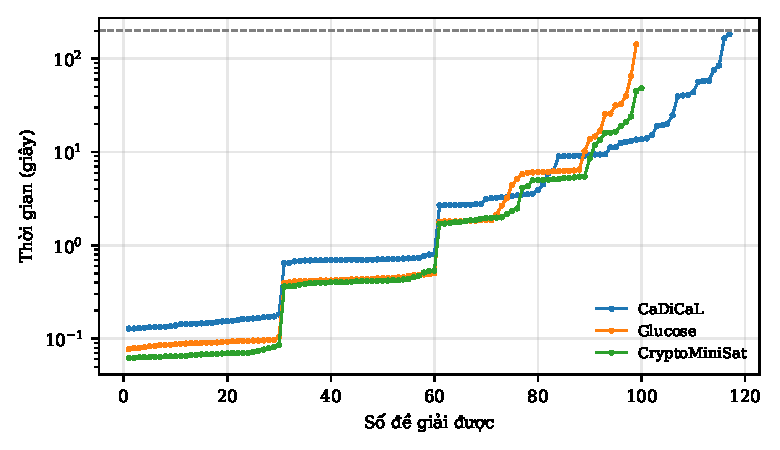
\includegraphics[width=0.75\linewidth]{figures/cactus.pdf}}{%
  \fbox{\parbox[c][4.2cm][c]{0.7\linewidth}{\centering\textcolor{red}{[Biểu đồ cactus: trục ngang là số đề giải được, trục dọc là thời gian, mỗi solver một đường. Lưu thành \texttt{figures/cactus.pdf} thì hình sẽ tự hiện ở đây.]}}}}
\caption{Biểu đồ cactus của các SAT solver với cấu hình \BestConfig{} trên toàn bộ dữ liệu. Đường càng thấp và càng dài về bên phải thì solver càng tốt.}
\label{fig:cactus}
\end{figure}

\subsection{Khả năng mở rộng}\label{sec:exp-scale}

\AutoScale{} Với $N=100$, CNF pairwise có khoảng $1{,}5\times10^8$ mệnh đề (Bảng~\ref{tab:size-min}), nên riêng bước sinh công thức bằng Python đã rất tốn thời gian và bộ nhớ.

\subsection{Hạn chế}\label{sec:threats}

Các đề tự sinh không nhất thiết có lời giải duy nhất, và cách xóa ô ngẫu nhiên không giống độ khó của các đề do người soạn; vì vậy ta thêm các bộ đề $9\times9$ đã công bố. SAT solver CDCL khá nhạy với thứ tự mệnh đề và biến, mà mỗi đề chỉ chạy một lần, nên kết quả trên từng đề có thể bị nhiễu. Encoder viết bằng Python nên với $N$ lớn thời gian sinh công thức đáng kể; cần ghi riêng thời gian sinh công thức và thời gian giải. Cuối cùng, các solver đều dùng tham số mặc định, nếu tinh chỉnh tham số thì thứ hạng có thể khác.

%% ============================================================================
\section{Conclusion}\label{sec:conclusion}

Trong bài tập lớn này ta đã xây dựng bộ giải Sudoku $N\times N$ dựa trên SAT. Ta trình bày hai cách mã hóa minimal và extended, giải thích vì sao chúng đúng, và kết hợp chúng với năm cách mã hóa AMO. Với mỗi cách, ta tính được số biến và số mệnh đề, đồng thời kiểm tra tính đúng và tính lan truyền bằng chương trình. Kết quả về kích thước cho thấy cách mã hóa AMO làm công thức thay đổi hơn một bậc độ lớn trên lưới lớn: ở $N=100$, mã hóa minimal có từ 8,71 triệu mệnh đề (product) đến 148,5 triệu mệnh đề (pairwise), còn trên lưới $9\times9$ thì sequential counter gọn nhất. \AutoConclusion

Hướng phát triển tiếp theo gồm: dùng commander và product nhiều tầng, thử cách mã hóa ``efficient'' (đơn giản hóa công thức bằng các ô cho trước trước khi giải), phá đối xứng khi sinh đề, dùng SAT tăng dần (incremental SAT) để đếm hoặc liệt kê lời giải, và so sánh thêm với các cách tiếp cận ILP và CP.

\section*{Declaration of competing interest}
Tác giả cam kết không có xung đột lợi ích tài chính hay quan hệ cá nhân nào có thể ảnh hưởng đến nội dung báo cáo.

\section*{Data availability}
Mã nguồn, dữ liệu, seed sinh đề và kết quả thô có tại \GithubURL.

%% ============================================================================
\appendix
\renewcommand{\thesection}{Appendix~\Alph{section}}

\section{Giải thích Mệnh đề~\ref{prop:amo} và~\ref{prop:up}}\label{app:proofs}

Với mỗi cách mã hóa, ta cần chỉ ra ba điều: (i) nếu có hai biến $x$ cùng đúng thì công thức bị vi phạm; (ii) nếu có nhiều nhất một $x$ đúng thì luôn chọn được giá trị cho các biến phụ để công thức đúng; (iii) gán $x_i=1$ thì UP suy ra mọi $x_j$ khác đều sai.

\paragraph{Pairwise.} Cả ba điều đều hiển nhiên: mệnh đề $(\neg x_i\vee\neg x_j)$ cấm hai biến cùng đúng và trở thành mệnh đề đơn ngay khi $x_i=1$.

\paragraph{Sequential counter.} (i) Nếu $x_i=x_j=1$ với $i<j$ thì $(\neg x_i\vee s_i)$ cho $s_i$, các mệnh đề $(\neg s_{k-1}\vee s_k)$ truyền tiếp đến $s_{j-1}$, và mệnh đề $(\neg x_j\vee\neg s_{j-1})$ bị vi phạm. (ii) Chọn $s_i=\bigvee_{k\le i}x_k$ thì mọi mệnh đề đều đúng. (iii) Từ $x_i=1$, UP suy ra $s_i,\dots,s_{m-1}$ rồi $\neg x_j$ với $j>i$; đồng thời suy ra $\neg s_{i-1}$, rồi $\neg s_{i-2},\dots,\neg s_1$, rồi $\neg x_j$ với $j<i$ qua $(\neg x_j\vee s_j)$.

\paragraph{Binary.} (i) Nếu $x_i$ và $x_j$ ($i\neq j$) cùng đúng thì mã của chúng khác nhau ở một bit $b$, nên hai mệnh đề ở bit $b$ đòi $y_b$ vừa đúng vừa sai. (ii) Gán $y$ bằng mã của biến đang đúng (nếu không biến nào đúng thì gán tùy ý). (iii) $x_i=1$ cố định mọi $y_b$; mỗi $x_j$ khác lệch ít nhất một bit nên mệnh đề tương ứng cho $\neg x_j$.

\paragraph{Commander.} (i) Hai biến đúng cùng nhóm thì vi phạm pairwise trong nhóm; khác nhóm $G_a\neq G_b$ thì ép $c_a=c_b=1$, vi phạm AMO trên các biến chỉ huy. (ii) Chọn $c_i=\bigvee G_i$. (iii) $x_i=1$ với $x_i\in G_a$ cho $c_a$, rồi $\neg c_b$ với $b\neq a$, rồi $\neg x$ cho mọi $x\in G_b$; trong $G_a$ thì pairwise cho $\neg x$.

\paragraph{Product.} (i) Hai biến đúng nằm ở hai vị trí khác nhau trên lưới $p\times q$, nên khác hàng (ép hai biến hàng cùng đúng) hoặc khác cột (ép hai biến cột cùng đúng), đều vi phạm. (ii) Chỉ gán đúng biến hàng và biến cột của biến đang đúng. (iii) $x_i=1$ cho $r_{u_i}$ và $c_{v_i}$, nên mọi biến hàng, cột khác đều sai; mỗi $x_j$ khác lệch hàng hoặc lệch cột nên bị suy ra sai.

Cuối cùng, vì phép gán $\{x_i=1\}$ luôn mở rộng được thành mô hình (theo (ii)) mà UP chỉ suy ra những literal bắt buộc, nên UP không thể gặp xung đột.

\section{Kích thước mã hóa extended}\label{app:tables}

\begin{table}[h]
\caption{Mã hóa extended (chưa tính ô cho trước): (a) số biến, (b) số mệnh đề. Giá trị nhỏ nhất trên mỗi hàng được in đậm.}
\label{tab:size-ext}
\centering\small
(a) Số biến\par\smallskip
\begin{tabular}{rrrrrr}
\toprule
$N$ & Pairwise & Sequential & Binary & Commander & Product \\
\midrule
9 & \textbf{729} & 3\,321 & 2\,025 & 1\,701 & 2\,673 \\
16 & \textbf{4\,096} & 19\,456 & 8\,192 & 10\,240 & 12\,288 \\
25 & \textbf{15\,625} & 75\,625 & 28\,125 & 38\,125 & 40\,625 \\
36 & \textbf{46\,656} & 228\,096 & 77\,760 & 108\,864 & 108\,864 \\
49 & \textbf{117\,649} & 578\,641 & 175\,273 & 280\,917 & 252\,105 \\
64 & \textbf{262\,144} & 1\,294\,336 & 360\,448 & 622\,592 & 524\,288 \\
100 & \textbf{1\,000\,000} & 4\,960\,000 & 1\,280\,000 & 2\,360\,000 & 1\,800\,000 \\
\bottomrule
\end{tabular}
\par\bigskip
(b) Số mệnh đề\par\smallskip
\begin{tabular}{rrrrrr}
\toprule
$N$ & Pairwise & Sequential & Binary & Commander & Product \\
\midrule
9 & 11\,988 & \textbf{7\,776} & 11\,988 & 8\,100 & 8\,100 \\
16 & 123\,904 & \textbf{46\,080} & 66\,560 & 53\,248 & \textbf{46\,080} \\
25 & 752\,500 & 180\,000 & 315\,000 & 235\,000 & \textbf{177\,500} \\
36 & 3\,271\,104 & 544\,320 & 1\,124\,928 & 782\,784 & \textbf{533\,952} \\
49 & 11\,303\,908 & 1\,382\,976 & 2\,833\,180 & 2\,401\,000 & \textbf{1\,354\,164} \\
64 & 33\,046\,528 & 3\,096\,576 & 6\,307\,840 & 6\,225\,920 & \textbf{3\,031\,040} \\
100 & 198\,040\,000 & 11\,880\,000 & 28\,040\,000 & 31\,760\,000 & \textbf{11\,640\,000} \\
\bottomrule
\end{tabular}

\end{table}

\section{Chạy lại kết quả}\label{app:repro}

Toàn bộ bảng và hình có thể sinh lại bằng các lệnh sau:
\begin{verbatim}
python sudoku_sat.py sizes  --out ../report  # Bang 2, 6, 11, Hinh 3
python sudoku_sat.py verify --out ../report  # Bang 7
python make_example_figure.py                # Hinh 2
python run_experiments.py run --profile full  # Bang 4,5,8,9, Hinh 4
\end{verbatim}
Kết quả từng lần chạy được lưu trong \texttt{results/runs.csv}.

\bibliographystyle{cas-model2-names}
\bibliography{sudoku-refs}

\end{document}
